\documentclass[twoside]{book}

% Packages required by doxygen
\usepackage{fixltx2e}
\usepackage{calc}
\usepackage{doxygen}
\usepackage{graphicx}
\usepackage[utf8]{inputenc}
\usepackage{makeidx}
\usepackage{multicol}
\usepackage{multirow}
\PassOptionsToPackage{warn}{textcomp}
\usepackage{textcomp}
\usepackage[nointegrals]{wasysym}
\usepackage[table]{xcolor}

% NLS support packages
\usepackage[french]{babel}

% Font selection
\usepackage[T1]{fontenc}
\usepackage{mathptmx}
\usepackage[scaled=.90]{helvet}
\usepackage{courier}
\usepackage{amssymb}
\usepackage{sectsty}
\renewcommand{\familydefault}{\sfdefault}
\allsectionsfont{%
  \fontseries{bc}\selectfont%
  \color{darkgray}%
}
\renewcommand{\DoxyLabelFont}{%
  \fontseries{bc}\selectfont%
  \color{darkgray}%
}
\newcommand{\+}{\discretionary{\mbox{\scriptsize$\hookleftarrow$}}{}{}}

% Page & text layout
\usepackage{geometry}
\geometry{%
  a4paper,%
  top=2.5cm,%
  bottom=2.5cm,%
  left=2.5cm,%
  right=2.5cm%
}
\tolerance=750
\hfuzz=15pt
\hbadness=750
\setlength{\emergencystretch}{15pt}
\setlength{\parindent}{0cm}
\setlength{\parskip}{0.2cm}
\makeatletter
\renewcommand{\paragraph}{%
  \@startsection{paragraph}{4}{0ex}{-1.0ex}{1.0ex}{%
    \normalfont\normalsize\bfseries\SS@parafont%
  }%
}
\renewcommand{\subparagraph}{%
  \@startsection{subparagraph}{5}{0ex}{-1.0ex}{1.0ex}{%
    \normalfont\normalsize\bfseries\SS@subparafont%
  }%
}
\makeatother

% Headers & footers
\usepackage{fancyhdr}
\pagestyle{fancyplain}
\fancyhead[LE]{\fancyplain{}{\bfseries\thepage}}
\fancyhead[CE]{\fancyplain{}{}}
\fancyhead[RE]{\fancyplain{}{\bfseries\leftmark}}
\fancyhead[LO]{\fancyplain{}{\bfseries\rightmark}}
\fancyhead[CO]{\fancyplain{}{}}
\fancyhead[RO]{\fancyplain{}{\bfseries\thepage}}
\fancyfoot[LE]{\fancyplain{}{}}
\fancyfoot[CE]{\fancyplain{}{}}
\fancyfoot[RE]{\fancyplain{}{\bfseries\scriptsize Généré le Mardi 20 Septembre 2016 14\+:36\+:26 pour My Project par Doxygen }}
\fancyfoot[LO]{\fancyplain{}{\bfseries\scriptsize Généré le Mardi 20 Septembre 2016 14\+:36\+:26 pour My Project par Doxygen }}
\fancyfoot[CO]{\fancyplain{}{}}
\fancyfoot[RO]{\fancyplain{}{}}
\renewcommand{\footrulewidth}{0.4pt}
\renewcommand{\chaptermark}[1]{%
  \markboth{#1}{}%
}
\renewcommand{\sectionmark}[1]{%
  \markright{\thesection\ #1}%
}

% Indices & bibliography
\usepackage{natbib}
\usepackage[titles]{tocloft}
\setcounter{tocdepth}{3}
\setcounter{secnumdepth}{5}
\makeindex

% Hyperlinks (required, but should be loaded last)
\usepackage{ifpdf}
\ifpdf
  \usepackage[pdftex,pagebackref=true]{hyperref}
\else
  \usepackage[ps2pdf,pagebackref=true]{hyperref}
\fi
\hypersetup{%
  colorlinks=true,%
  linkcolor=blue,%
  citecolor=blue,%
  unicode%
}

% Custom commands
\newcommand{\clearemptydoublepage}{%
  \newpage{\pagestyle{empty}\cleardoublepage}%
}


%===== C O N T E N T S =====

\begin{document}

% Titlepage & ToC
\hypersetup{pageanchor=false,
             bookmarks=true,
             bookmarksnumbered=true,
             pdfencoding=unicode
            }
\pagenumbering{roman}
\begin{titlepage}
\vspace*{7cm}
\begin{center}%
{\Large My Project }\\
\vspace*{1cm}
{\large Généré par Doxygen 1.8.7}\\
\vspace*{0.5cm}
{\small Mardi 20 Septembre 2016 14:36:26}\\
\end{center}
\end{titlepage}
\clearemptydoublepage
\tableofcontents
\clearemptydoublepage
\pagenumbering{arabic}
\hypersetup{pageanchor=true}

%--- Begin generated contents ---
\chapter{Liste des tests}
\label{test}
\hypertarget{test}{}

\begin{DoxyRefList}
\item[\label{test__test000001}%
\hypertarget{test__test000001}{}%
Membre \hyperlink{tp1-1_8cpp_ae66f6b31b5ad750f1fe042a706a4e3d4}{main} ()]\begin{TabularC}{4}
\hline
\rowcolor{lightgray}{\bf Entrees }&{\bf Sorties }&{\bf Justification }&{\bf Resultat  }\\\cline{1-4}
n=1 &m=1 &branche alors &passe \\\cline{1-4}
n=0 &m=0 &cas limite &passe \\\cline{1-4}
n=-\/1 &m=1 &branche sinon &passe \\\cline{1-4}
n='a' &E\+R\+R\+E\+U\+R &illicite &échoue (problème de saisie C++) \\\cline{1-4}
\end{TabularC}

\end{DoxyRefList}
\chapter{Index des fichiers}
\section{Liste des fichiers}
Liste de tous les fichiers documentés avec une brève description \+:\begin{DoxyCompactList}
\item\contentsline{section}{\hyperlink{tp1-1_8cpp}{tp1-\/1.\+cpp} \\*Programme implémentant l'algorithme de calcul de la valeur absolue vu en C\+M }{\pageref{tp1-1_8cpp}}{}
\end{DoxyCompactList}

\chapter{Documentation des fichiers}
\hypertarget{tp1-1_8cpp}{\section{Référence du fichier tp1-\/1.cpp}
\label{tp1-1_8cpp}\index{tp1-\/1.\+cpp@{tp1-\/1.\+cpp}}
}


Programme implémentant l'algorithme de calcul de la valeur absolue vu en C\+M.  


{\ttfamily \#include $<$iostream$>$}\\*
{\ttfamily \#include $<$cassert$>$}\\*
{\ttfamily \#include $<$cmath$>$}\\*
Graphe des dépendances par inclusion de tp1-\/1.cpp\+:
\nopagebreak
\begin{figure}[H]
\begin{center}
\leavevmode
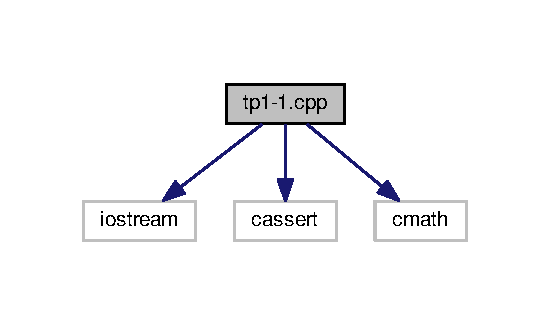
\includegraphics[width=264pt]{tp1-1_8cpp__incl}
\end{center}
\end{figure}
\subsection*{Fonctions}
\begin{DoxyCompactItemize}
\item 
int \hyperlink{tp1-1_8cpp_ae66f6b31b5ad750f1fe042a706a4e3d4}{main} ()
\begin{DoxyCompactList}\small\item\em fonction principale \end{DoxyCompactList}\end{DoxyCompactItemize}


\subsection{Description détaillée}
Programme implémentant l'algorithme de calcul de la valeur absolue vu en C\+M. 

\begin{DoxyAuthor}{Auteur}
C. Jermann 
\end{DoxyAuthor}
\begin{DoxyDate}{Date}
15/09/2015 Création 

15/09/2016 Actualisation du commentaire d'entête 
\end{DoxyDate}


Définition dans le fichier \hyperlink{tp1-1_8cpp_source}{tp1-\/1.\+cpp}.



\subsection{Documentation des fonctions}
\hypertarget{tp1-1_8cpp_ae66f6b31b5ad750f1fe042a706a4e3d4}{\index{tp1-\/1.\+cpp@{tp1-\/1.\+cpp}!main@{main}}
\index{main@{main}!tp1-\/1.\+cpp@{tp1-\/1.\+cpp}}
\subsubsection[{main}]{\setlength{\rightskip}{0pt plus 5cm}int main (
\begin{DoxyParamCaption}
{}
\end{DoxyParamCaption}
)}}\label{tp1-1_8cpp_ae66f6b31b5ad750f1fe042a706a4e3d4}


fonction principale 

{\bfseries Role} \+: calculer la valeur absolue d'un entier saisi par l'utilisateur

{\bfseries Entrée} \+:
\begin{DoxyItemize}
\item {\itshape n} entier positif
\end{DoxyItemize}

{\bfseries Sortie} \+:
\begin{DoxyItemize}
\item {\itshape m} valeur absolue de n
\end{DoxyItemize}

\begin{DoxyPrecond}{Précondition}
Entier n
\end{DoxyPrecond}
\begin{DoxyPostcond}{Postcondition}
m=$\vert$n$\vert$
\end{DoxyPostcond}
\begin{DoxyRefDesc}{Test}
\item[\hyperlink{test__test000001}{Test}]\begin{TabularC}{4}
\hline
\rowcolor{lightgray}{\bf Entrees }&{\bf Sorties }&{\bf Justification }&{\bf Resultat  }\\\cline{1-4}
n=1 &m=1 &branche alors &passe \\\cline{1-4}
n=0 &m=0 &cas limite &passe \\\cline{1-4}
n=-\/1 &m=1 &branche sinon &passe \\\cline{1-4}
n='a' &E\+R\+R\+E\+U\+R &illicite &échoue (problème de saisie C++) \\\cline{1-4}
\end{TabularC}
\end{DoxyRefDesc}


Ce programme demande à l'utilisateur un entier et en calcule la valeur absolue au moyen d'une conditionnelle, puis affiche le résultat. Il illustre la documentation Doxygen d'un programme et l'utilisation des assertions. 

Définition à la ligne 43 du fichier tp1-\/1.\+cpp.


%--- End generated contents ---

% Index
\newpage
\phantomsection
\addcontentsline{toc}{chapter}{Index}
\printindex

\end{document}
